\documentclass[12pt,a4paper]{scrartcl}

\author{Sebastian Hirnschall}
%% (C) Hirnschall Sebastian 2016 
\date{\today}

\usepackage[hidelinks]{hyperref}
\hypersetup{
	pdftitle={Designing Circular and Non-Circular Gears for FDM 3d-Printing},
	pdfsubject={Designing Circular and Non-Circular Gears for FDM 3d-Printing},
	pdfauthor={Sebastian Hirnschall},
	pdfkeywords={gears, circular, non-circular, fdm, fff, sla, 3d-printing}
}


\usepackage[
backend=biber,
style=authoryear-icomp,    % Zitierstil
isbn=false,                % ISBN nicht anzeigen, gleiches geht mit nahezu allen anderen Feldern
pagetracker=true,          % ebd. bei wiederholten Angaben (false=ausgeschaltet, page=Seite, spread=Doppelseite, true=automatisch)
maxbibnames=50,            % maximale Namen, die im Literaturverzeichnis angezeigt werden (ich wollte alle)
maxcitenames=3,            % maximale Namen, die im Text angezeigt werden, ab 4 wird u.a. nach den ersten Autor angezeigt
autocite=inline,           % regelt Aussehen für \autocite (inline=\parancite)
block=space,               % kleiner horizontaler Platz zwischen den Feldern
backref=true,              % Seiten anzeigen, auf denen die Referenz vorkommt
backrefstyle=three+,       % fasst Seiten zusammen, z.B. S. 2f, 6ff, 7-10
date=short                % Datumsformat
]{biblatex}

\addbibresource{refs.bib}

\usepackage{longtable}
%\usepackage{hyperref}
\usepackage{amsmath}% http://ctan.org/pkg/amsmath
\usepackage[english]{cleveref} %referenzen fur Abbildungen
\usepackage{graphicx}
\usepackage{listings}
\usepackage{esdiff}
\usepackage[utf8]{inputenc}
\usepackage[english]{babel}
\usepackage[T1]{fontenc}
\usepackage{graphicx}
\usepackage{amssymb}
\usepackage{geometry}% http://ctan.org/pkg/geometry
\usepackage{amsthm}
\usepackage{tocloft}
\usepackage{framed}
\usepackage{mathtools}
\usepackage{color}
\usepackage{multirow}
\usepackage{textcomp}
\usepackage{subcaption}
\usepackage{float}
%\usepackage[dvipsnames]{xcolor}
\usepackage[ruled,vlined]{algorithm2e}
\usepackage{csquotes}


\usepackage[table,xcdraw,dvipsnames]{xcolor}

\usepackage{fancyvrb}

\usepackage{tikz}
\usetikzlibrary{spy}
\usetikzlibrary{calc,arrows}

% redefine \VerbatimInput
\RecustomVerbatimCommand{\VerbatimInput}{VerbatimInput}%
{fontsize=\footnotesize,
	%
	frame=lines,  % top and bottom rule only
	framesep=2em, % separation between frame and text
	rulecolor=\color{Gray},
	%
	label=\fbox{\color{Black}yahoo-stats.txt},
	labelposition=topline,
	%
}


%change title font
%\usepackage{titlesec}
%\setkomafont{\section}{\LARGE\bfseries}
%\setkomafont{\subsection}{\Large\bfseries}
%\setkomafont{\subsubsection}{\large\bfseries}
%\setkomafont{\paragraph}{\large\bfseries}
%\setkomafont{\subparagraph}{\large\bfseries}




%\pagestyle{headings}

\setcounter{secnumdepth}{5}
\setcounter{tocdepth}{5}

%\pagestyle{headings}

\usepackage{fancyhdr}
\pagestyle{fancy}
%
\rhead{ \rightmark}
%\rhead[re]{\textbf{\nouppercase{\leftmark}}}
\chead{}
\lhead{}
%%
\lfoot{Sebastian Hirnschall}
\cfoot{}
\rfoot{\thepage}
%%
\renewcommand{\headrulewidth}{0.2pt}
\renewcommand{\footrulewidth}{0.2pt}


\fancypagestyle{firststyle}
{
	\fancyhf{}
	\rhead{}
	%\rhead[re]{\textbf{\nouppercase{\leftmark}}}
	\chead{}
	\lhead{}
	\lfoot{ Sebastian Hirnschall}
	\cfoot{}
	\rfoot{\thepage}
}


%listings settings
\definecolor{mygreen}{rgb}{0,0.6,0}
\definecolor{mygray}{rgb}{0.5,0.5,0.5}
\definecolor{mymauve}{rgb}{0.58,0,0.82}
\definecolor{BackgroundGray}{rgb}{0.9,0.9,0.9}

\lstset{ %
	backgroundcolor=\color{BackgroundGray},   % choose the background color; you must add \usepackage{color} or \usepackage{xcolor}
	basicstyle=\footnotesize,        % the size of the fonts that are used for the code
	breakatwhitespace=false,         % sets if automatic breaks should only happen at whitespace
	breaklines=true,                 % sets automatic line breaking
	captionpos=b,                    % sets the caption-position to bottom
	commentstyle=\color{mygreen},    % comment style
	deletekeywords={...},            % if you want to delete keywords from the given language
	escapeinside={\%*}{*)},          % if you want to add LaTeX within your code
	extendedchars=true,              % lets you use non-ASCII characters; for 8-bits encodings only, does not work with UTF-8
	frame=single,	                   % adds a frame around the code
	keepspaces=true,                 % keeps spaces in text, useful for keeping indentation of code (possibly needs columns=flexible)
	keywordstyle=\color{blue},       % keyword style
	language=C,                 	   % the language of the code
	otherkeywords={*,...},           % if you want to add more keywords to the set
	numbers=left,                    % where to put the line-numbers; possible values are (none, left, right)
	numbersep=5pt,                   % how far the line-numbers are from the code
	numberstyle=\tiny\color{mygray}, % the style that is used for the line-numbers
	rulecolor=\color{mygray},         % if not set, the frame-color may be changed on line-breaks within not-black text (e.g. comments (green here))
	showspaces=false,                % show spaces everywhere adding particular underscores; it overrides 'showstringspaces'
	showstringspaces=false,          % underline spaces within strings only
	showtabs=false,                  % show tabs within strings adding particular underscores
	stepnumber=2,                    % the step between two line-numbers. If it's 1, each line will be numbered
	stringstyle=\color{mymauve},     % string literal style
	tabsize=2,	                   % sets default tabsize to 2 spaces
	title=\lstname,                   % show the filename of files included with \lstinputlisting; also try caption instead of title
	emph={int,unsigned,long,vector,char,string},
	emphstyle={\color{ForestGreen}}
}

%italic quotes
\newenvironment{italicquotes}
{\begin{quote}\itshape}
	{\end{quote}}


%tableofcontents font
%\renewcommand{\cftchapfont}{\scshape}
\renewcommand{\cftsecfont}{\bfseries}
\addtokomafont{disposition}{\rmfamily}

\newcommand{\spar}{\par\vspace{10pt}\noindent}
\newcommand{\Mod}[1]{\ (\text{mod}\ #1)}

\usepackage{twoopt}
\newcommandtwoopt{\img}[4][0.5cm][0.7]{
	\begin{figure}[!h]
		\vspace{#1}
		\centering
		\includegraphics[width=#2\textwidth]{images/#3}
		\caption{#4} %\footnotemark}
		\label{fig:#3}
	\end{figure}
	%\footnotetext{#5}
}




\numberwithin{equation}{section} 
%\makeatletter
%\@addtoreset{equation}{section}
%\makeatother



%\newtheorem{theorem}{Theorem}[section]
%\newtheorem{lemma}[theorem]{Lemma}
%\newtheorem{proposition}[theorem]{Proposition}
%\newtheorem{corollary}[theorem]{Corollary}

\newcounter{myalgctr}

\newenvironment{mydefinition}{%      define a custom environment
	\bigskip\noindent%         create a vertical offset to previous material
	\refstepcounter{myalgctr}% increment the environment's counter
	\textsc{\textbf{Definition} \themyalgctr}% or \textbf, \textit, ...
	\newline
}{\par\bigskip}  %          create a vertical offset to following material
\numberwithin{myalgctr}{section}

\crefname{myalgctr}{Definition}{Definitions}

\newcounter{mytheoremctr}

\newenvironment{mytheorem}{%      define a custom environment
	\bigskip\noindent%         create a vertical offset to previous material
	\refstepcounter{mytheoremctr}% increment the environment's counter
	\textsc{\textbf{Theorem} \themytheoremctr}% or \textbf, \textit, ...
	\newline
}{\par\bigskip}  %          create a vertical offset to following material
\numberwithin{mytheoremctr}{section}

\crefname{mytheoremctr}{Theorem}{Theorems}

\newenvironment{myproof}{%      define a custom environment
	\bigskip\noindent%         create a vertical offset to previous material
	\textsc{\textbf{Proof}}% or \textbf, \textit, ...
	\indent
}{\qed\par\bigskip}  %          create a vertical offset to following material



\newcounter{myexamplectr}

\newcommand{\myexample}[1]{
	\par\noindent
	\addcontentsline{toc}{subsubsection}{#1}
	\refstepcounter{myexamplectr}
	\textsc{\textbf{Example \themyexamplectr}}\ #1
	\par}
\numberwithin{myexamplectr}{subsection}

\crefname{myexamplectr}{example}{examples}

%\renewenvironment{proof}[1][Beweis]{\begin{trivlist}
%		\item[\hskip \labelsep {\bfseries #1}]}{\end{trivlist}}
%\newenvironment{example}[1][Beispiel]{\begin{trivlist}
%		\item[\hskip \labelsep {\bfseries #1}]}{\end{trivlist}}
%\newenvironment{remark}[1][Remark]{\begin{trivlist}
%		\item[\hskip \labelsep {\bfseries #1}]}{\end{trivlist}}

%\renewcommand{\qed}{\nobreak \ifvmode \relax \else
%	\ifdim\lastskip<1.5em \hskip-\lastskip
%	\hskip1.5em plus0em minus0.5em \fi \nobreak
%	\vrule height0.75em width0.5em depth0.25em\fi}

\newcommand{\mpar}[1]{\paragraph*{#1}\mbox{}\par}

\usepackage{makeidx}
\makeindex
\newcommand{\ind}[1]{\textit{#1}\index{#1}}

\usepackage{breqn}


\begin{document}
	\newgeometry{bottom=1cm,top=7.5cm}
	\begin{titlepage}
		\centering
		\vspace{10cm}
		{\huge\bfseries Designing Circular and Non-Circular Gears for FDM 3d-Printing\par}
		\vspace{2cm}
		{\Large\itshape Sebastian Hirnschall\par}
		\vspace{3cm}
		\begin{figure}[!h]
			\vspace{0cm}
			\centering
			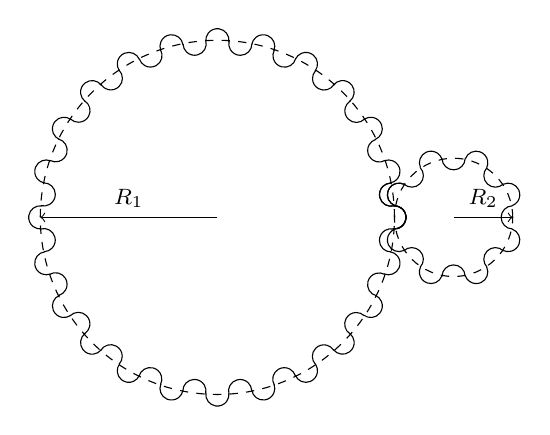
\begin{tikzpicture}[x=1mm,y=1mm]
			\coordinate (m1) at (0,0);
			\coordinate (m2) at (30,0);
			%\path (m1)  + ({22.49085405 * cos(0)},{22.49085405 * sin(0)}) arc[radius = 22.49085405, start angle=0,end angle =360] coordinate[pos=0] (km1) ;
			\draw[dashed] (m1)  + ({22.49085405 * cos(0)},{22.49085405 * sin(0)}) arc[radius = 22.49085405, start angle=0,end angle =360] coordinate[pos={8/360}] (km2) ;
			\draw[dashed] (m2)  + ({7.508037642 * cos(0)},{7.508037642 * sin(0)}) arc[radius = 7.508037642, start angle=0,end angle =360] ;
			%big gear
			\foreach \i in {0,1, ...,24}{
				\begin{scope}[rotate around={\i*15:(m1)}]
				%nach aussen
				\draw (22.49196236,0) + ({1.471832758 * cos(-97.87500000)},{1.471832758 * sin(-97.87500000)}) arc[radius=1.471832758,start angle = -97.87500000,end angle = 95.87500000];
				%nach innen
				\draw ({22.49196236*cos(7.5)},{22.49196236*sin(7.5)}) + ({1.471832758 * cos(-84)},{1.471832758 * sin(-84)}) arc[radius=1.471832758,start angle = -74.37500000,end angle = -268.125];
				\end{scope}
			}
			
			%small gear
			\foreach \i in {0,1, ...,8}{
				\begin{scope}[rotate around={\i*45:(m2)}]
				%nach aussen
				\draw (22.49196236,0) + ({1.471832758 * cos(-88.62500000)},{1.471832758 * sin(-88.62500000)}) arc[radius=1.471832758,start angle = -88.62500000,end angle = 88.62500000];
				%nach innen
				\draw (m2) ++ ({180-45/2}:7.508037642) ++ ({1.471832758 * cos(-110.12500000)},{1.471832758 * sin(-110.12500000)}) arc[radius=1.471832758,start angle = -110.12500000,end angle = -294.875];
				\end{scope}
			}
				
			%radii
			\draw[->] (m1) -- +(-22.49196236,0) node[pos=0.5,above] {\footnotesize$R_1$};
			\draw[->] (m2) -- +(7.508037642,0) node[pos=0.5,above] {\footnotesize$R_2$};		
			\end{tikzpicture}
		\end{figure}
		
		\vfill
		
		% Bottom of the page
		{\large \today\par}
	\end{titlepage}
	\restoregeometry
	
	\thispagestyle{firststyle}

	\newpage
	\tableofcontents
	\thispagestyle{firststyle}
	
	\newpage
	\section{Tooth Profile}
		Since FDM 3d printed gears are weak and therefore torque and transmission efficiency is not as important we are going to use a circular \ind{tooth profile}. Please note that this profile is not optimal but it makes it incredibly easy to calculate and draw non circular gears. It is sufficient for most 3d printed parts. If this is not suitable for your design take a look at involute gears.\\
		\begin{figure}[!h]
			\centering
%		\begin{tikzpicture}[scale=1]
%			\draw[gray,dashed,thick] (0,0) arc[radius=5cm,start angle=44,end angle =136];
%			\path (0,0) arc[radius=5cm,start angle=44,end angle =136] node[pos=0.5] (A) {};
%			\path (0,0) arc[radius=5cm,start angle=44,end angle =136] node[pos=0.25] (B) {};
%			\path (0,0) arc[radius=5cm,start angle=44,end angle =136] node[pos=0.75] (C) {};
%			\path (0,0) arc[radius=5cm,start angle=44,end angle =136] node[pos=0] (D) {};
%			\path (0,0) arc[radius=5cm,start angle=44,end angle =136] node[pos=1] (E) {};
%			%middle circle:
%			\draw[gray,ultra thick] (A)+(0,1) arc[radius=1cm,start angle=90,end angle =185.73917045];
%			\draw[gray,ultra thick] (A)+(0,1) arc[radius=1cm,start angle=90,end angle =-5.73917045];		
%			\draw[gray,dashed,thick] (A)+(0,-1) arc[radius=1cm,start angle=-90,end angle =-174.2608296];		
%			\draw[gray,dashed,thick] (A)+(0,-1) arc[radius=1cm,start angle=-90,end angle =-5.73917045];
%			
%			%right circle:
%			\draw[gray,dashed,thick] (B)+({cos(-28.73917045)},{sin(-28.73917045)}) arc (-28.73917045:162.73917045:1);
%			\draw[gray,ultra thick] (B)+({cos(-28.73917045)},{sin(-28.73917045)}) arc (-28.73917045:-197.26082955:1);
%			
%			%left circle
%			\draw[gray,dashed,thick] (C)+({cos(17.26082955)},{sin(17.26082955)}) arc (17.26082955:208.73917045:1);
%			\draw[gray,ultra thick] (C)+({cos(17.26082955)},{sin(17.26082955)}) arc (17.26082955:-151.26082955:1);
%			
%			
%			%right most circle:
%			\draw[gray,ultra thick] (D)+({cos(46.73917045)},{sin(46.73917045)}) arc (46.73917045:139.73917045:1);
%			\draw[gray,dashed] (D)+({cos(-134.73917045)},{sin(-134.73917045)}) arc (-134.73917045:-220.26082955:1);
%			
%			%left most circle:
%			\draw[gray,ultra thick] (E)+({cos(39.73917045)},{sin(39.73917045)}) arc (39.73917045:133.73917045:1);
%			\draw[gray,dashed] (E)+({cos(-44.73917045)},{sin(-44.73917045)}) arc (-44.73917045:46.26082955:1);
%			
%			\coordinate (O) at ($(A)+(0,-5)$);
%			
%			\draw[gray,ultra thick,dashed] (O) -- ($(O)!6cm!(D)$);
%			\draw[gray,ultra thick,dashed] (O) -- ($(O)!6cm!(E)$);
%			
%		\end{tikzpicture}
		\begin{tikzpicture}[x=1mm,y=1mm,spy using outlines=
		{circle, magnification=4, connect spies}]
		\draw[dashed] (0,0)  + ({22.49085405 * cos(0)},{22.49085405 * sin(0)}) arc[radius = 22.49085405, start angle=0,end angle =360];
		
			%big gear
			\foreach \i in {0,1, ...,24}{
				\begin{scope}[rotate around={\i*15:(m1)}]
				%nach aussen
				\draw (22.49196236,0) + ({1.471832758 * cos(-97.87500000)},{1.471832758 * sin(-97.87500000)}) arc[radius=1.471832758,start angle = -97.87500000,end angle = 95.87500000];
				%nach innen
				\draw ({22.49196236*cos(7.5)},{22.49196236*sin(7.5)}) + ({1.471832758 * cos(-84)},{1.471832758 * sin(-84)}) arc[radius=1.471832758,start angle = -74.37500000,end angle = -268.125];
				\end{scope}
			}
		\draw[->] (0,0) -- +(-22.49196236,0) node[pos=0.5,above] {\footnotesize$R_1$};
		

		%zoom
		\spy[size=4cm] on (22.49196236,0) in node (zoom) [left] at (70,0);
		\end{tikzpicture}
		\caption{Gear profile construction using circles}
		\end{figure}
		%abbidung close up 3 zaehne
	
	\subsection{Drawing a Gear}\label{sec:drawing}
	Start by drawing the outline of the gear. As we will see in \cref{non-circular} this can be any convex shape. As an example we will take a look at a circular gear. Then, using a compass, mark points with distance $r$ on the outline of your shape and draw a circle with radius $r$ on every second mark. We will see in \cref{section-gears} and in the examples how to calculate $r$.
	\begin{figure}[h!]
			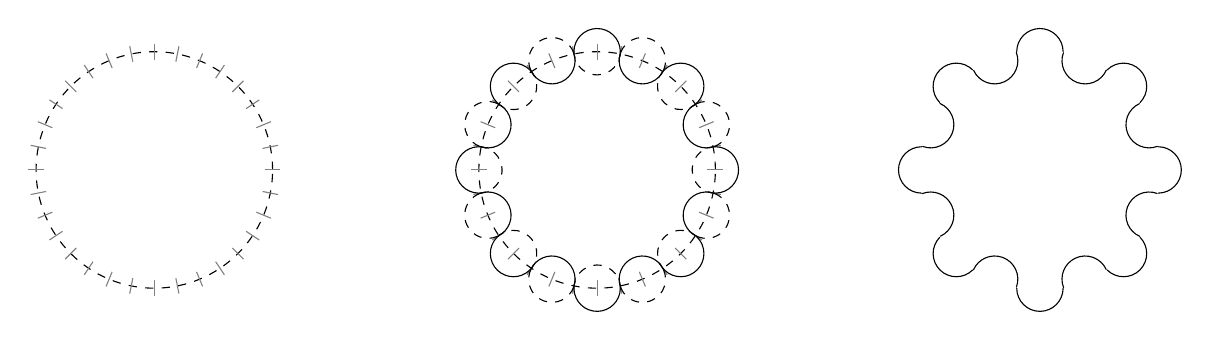
\begin{tikzpicture}[x=1mm,y=1mm,scale = 2]
			\draw[dashed] (0,0) circle[radius = 7.508037642];
			\foreach \i in {0,1,...,31}
			{
				\begin{scope}[rotate=\i*360/32]
				\draw[gray] (7.008037642,0) -- (8.008037642,0);
				\end{scope}
			}
		\begin{scope}[xshift=80]
			\draw[dashed] (0,0) circle[radius = 7.508037642];
			\foreach \i in {0,1,...,31}
			{
				\begin{scope}[rotate=\i*360/32]
				\draw[gray] (7.008037642,0) -- (8.008037642,0);
				\end{scope}
			}
			\foreach \i in {0,1,...,7}
			{
				\begin{scope}[rotate=\i*360/8]
				
				%nach aussen
				\draw (7.508037642,0) + ({1.471832758 * cos(-88.62500000)},{1.471832758 * sin(-88.62500000)}) arc[radius=1.471832758,start angle = -88.62500000,end angle = 88.62500000];
				\draw[dashed] (7.508037642,0) + ({1.471832758 * cos(-88.62500000)},{1.471832758 * sin(-88.62500000)}) arc[radius=1.471832758,start angle = -88.62500000,end angle = -271.375];
				%nach innen
				\draw[dashed] (0,0) ++ ({180-45/2}:7.508037642) ++ ({1.471832758 * cos(-110.12500000)},{1.471832758 * sin(-110.12500000)}) arc[radius=1.471832758,start angle = -110.12500000,end angle = -294.875];
				\draw (0,0) ++ ({180-45/2}:7.508037642) ++ ({1.471832758 * cos(-110.12500000)},{1.471832758 * sin(-110.12500000)}) arc[radius=1.471832758,start angle = -110.12500000,end angle = 66.125];
				
				
				\end{scope}
			}
			\end{scope}
			
			\begin{scope}[xshift=160]
			\foreach \i in {0,1,...,7}
			{
				\begin{scope}[rotate=\i*360/8]
				
				%nach aussen
				\draw[line cap=round] (7.508037642,0) + ({1.471832758 * cos(-89.62500000)},{1.471832758 * sin(-89.62500000)}) arc[radius=1.471832758,start angle = -89.62500000,end angle = 89.62500000];
				%nach innen
				\draw[line cap=round] (0,0) ++ ({180-45/2}:7.508037642) ++ ({1.471832758 * cos(-110.12500000)},{1.471832758 * sin(-110.12500000)}) arc[radius=1.471832758,start angle = -110.12500000,end angle = 66.125];
				
				
				\end{scope}
			}
			\end{scope}
		\end{tikzpicture}
		\caption{Drawing a circular gear}
	\end{figure}
	
	\newpage
	\section{Notation}
	To analyze different gear shapes and calculate the \ind{tooth size} $r$ we need to grasp what a gear is mathematically. As seen in the previous chapter, a gear is constituted by the \ind{gear shape} together with the number of teeth, the size (radius) of each tooth, a set containing the centerpoints of each tooth and the \ind{centerpoint} of the gear itself. This leads to the following definition:
	
	
	\begin{mydefinition}\label{def:gear1}
		\index{$\gamma$}\index{$n$}\index{$r$}\index{$m_0$}\index{$(m_i)_{i\in\mathbb{Z}_{2n}}$}\index{$M$}
		Let $\gamma:[0,2\pi]\mapsto\mathbb{R}^2$ be a simple, closed and rectifiable curve such that a convex domain $\Omega$ with $\partial\Omega = \gamma[[0,2\pi]]$ exists.\\
		We'll call a tuple $(\gamma, n, m_0, M)$ where $n\in\mathbb{N}$ a \ind{gear} if it is possible to find a polygon $\Gamma$ with $4n$ vertices $(m_i)_{i\in\mathbb{Z}_{4n}}\in\gamma[[0,2\pi]]$ such that $\exists!r\in\mathbb{R}\forall i\in\mathbb{Z}_{4n}:d(m_i,m_{i+1})=r\land r>0$. 
	\end{mydefinition}

	At this point it is not clear if a gear is well-defined as \cref{def:gear1} demands only a single tooth-centerpoint $m_0$ and not a set containing every tooth-centerpoint. The fact that $(m_i)_{i\in\mathbb{Z}_{4n}}$ can be represented by $m_0$ is one of the findings of \cref{theorem:non-circular}.
	\newline
	If $\gamma$ is a circle we will sometimes replace it with its radius $R\in\mathbb{R}$.
	Furthermore $M$ is defined as the center point of $\Omega$. $M\coloneqq\frac{1}{\lambda^2(\Omega)}\int_{\Omega}xd\lambda^2$.
	Since $M$ is defined by $\gamma$ it is not required. However we will only omit $M$ if it is $0$.
	
	\begin{mydefinition}
		Two gears $A$ and $B$ \ind{fit together} if 
		\begin{align*}
		r_A=r_B.
		\end{align*}
	\end{mydefinition}
	
	\begin{mydefinition}\label{def:rel}
		Two gears $A$ and $B$ are of the \ind{same size} or shape, if it is possible to map the image of $\gamma_A$ to the image of $\gamma_B$ without changing its size:
		\begin{align}
		\exists\iota (\forall x,y\in\mathbb{R}^2: d(\iota(x),\iota(y))=d(x,y))\land(\iota[\gamma_A[[0,2\pi)]] = \gamma_B[[0,2\pi)]).\label{imp:sim}
		\end{align}
		We call two gears $A$ and $B$ \ind{similar}\index{$\sim$} and write $A\sim B$ if they are of the same size and
		\begin{gather*}
		n_A=n_B\\
		r_A=r_B\\
		\iota(m_{A,0}) = m_{B,0}
		\end{gather*}
		where $\iota$ is an isometric function that satisfies \eqref{imp:sim}.\\
		Furthermore $A=B$\index{$=$} if $A\sim B$ and $\iota=\text{id}$.
%		As $d(m_i,m_{i+1})=r$, $(m_{A,i})_{i\in\mathbb{Z}_{2n_A}}$ is defined by $m_0$ and $r$ and therefore
%		\begin{align*}
%			\iota(m_{A,0}) = m_{B,0}\implies\iota[(m_{A,i})_{i\in\mathbb{Z}_{2n_A}}] = (m_{B,j})_{j\in\mathbb{Z}_{2n_B}}.
%		\end{align*}
		
	\end{mydefinition}

	\begin{myproof}
		
		
		For this definition to make sense $\sim$ needs to be reflexive, symmetric and transitive.\\
		{ "$A\sim A$":}\par
		Let $\iota$ be the identity function.\\
		{ "$A\sim B\implies B\sim A$":}\par
		As $\iota$ is an isometric function it is injective and therefore its left inverse $\iota^{-1}$ exists. Using $\iota^{-1}$, $B\sim A$.\\
		{ "$A\sim B\land B\sim C\implies A\sim C$":}\par
		The composition of two isometric functions is an isometric function and therefore $A\sim C$.
	\end{myproof}
	
	\newpage
	\section{Calculating Gear and teeth Size}\label{section-gears}
	\subsection{Circular Gears}\label{section-circ}
	%Designing a circular gear is straightforward. We start by drawing a circle $K$ with radius $R$. This will be the size of our final gear. We then look for a sequence of smaller circles $(k_i)_{i\in I}$ with radius $r$ such that their center is on $K$, they intersect each other on $K$, they cover $K$ completely and the number of $k_i$ must be even ($|I|=2n : n\in \mathbb{N}$). This is important since the number of teeth has to be a positive integer. 
	
	We have already seen how to draw a circular gear $K=(R,n,m_0,M)$ in \cref{sec:drawing}. However $r$ has to be chosen in a way that it is possible to find a set of $4n$ points $(m_i)_{i\in\mathbb{Z}_{4n}}\in\gamma[[0,2\pi)]:d(m_i,m_{i+1})=r\land r>0$.
	
	%abbildung kreise auf dem kreis
	
	
	\begin{mytheorem}\label{theorem-circle}
		Given a circle $K$ with radius $R$, $(R,n\in\mathbb{N}^*,m_0\in K,M)$ is a gear. Let $\varphi = \frac{\pi}{n}$ then
		\begin{align}
		r= \frac{R\cdot\sin\left( \varphi\right) }{\cos(\frac{\varphi}{2})}.\label{eq:R-r}
		\end{align}
	\end{mytheorem}

	\begin{myproof}
		
		Let $K$ be a circle with radius $R$ and center $(0,0)$ and $n\in\mathbb{N}^*$ we can, using polar coordinates, construct a sequence $(m_i)_{i\in\mathbb{Z}_{4n}}$, $m_i = \left(R,i\cdot\frac{\pi}{2n}\text{rad}\right)$ of $4n$ points on $K$. They are evenly spaced and $r\coloneqq d(m_1,m_2)$.
		
		%constructing the small circles k_j
		%We can now construct a sequence $(k_j)_{j\in\mathbb{Z}_n}$of $n$ circles with radius $r$ and center $m_j:j\equiv 0 \Mod 2$. Therefore $\{x\in K:\exists i,j\in \mathbb{Z}_{2n}: d(x,m_{2i})\leq r\land d(x,m_{2j})\leq r\} = \{m_i:i\equiv 1 \Mod 2,i\in\mathbb{Z}_{2n}\}$ and $|\{m_i:i\equiv 1 \Mod 2,i\in\mathbb{Z}_{2n}\}| = n$.
		
		\begin{figure}[h!]
			\centering
			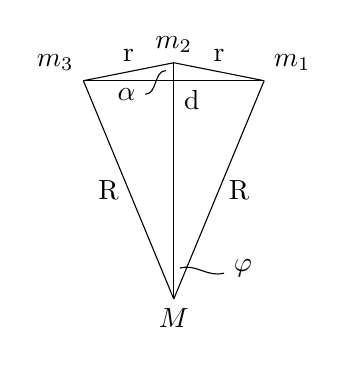
\begin{tikzpicture}[x=1mm,y=1mm,scale = 2]
				\draw (0,0) -- (90:15);
				\draw (0,0) -- (112.5:15) node[pos=0.5,left] {R};
				\draw (0,0) -- (67.5:15) node[pos=0.5,right] {R};
				\draw (90:15) -- (67.5:15) node[pos=0.5,above] {r};
				\draw (90:15) -- (112.5:15) node[pos=0.5,above] {r};
				\draw (67.5:15) -- (112.5:15) node[pos=0.4,below]{d};
				%phi
				\node (phi) at ($(78.75:2) + (4,0) $) {$\varphi$};
				\draw (78.75:2) to[out=15,in=195] (phi);
				%\draw (67.5:3) arc[radius = 3, start angle=67.5,end angle =112.5];
				%alpha
				\node (alpha) at ($(90:15) + (2,-2)  + (-5,0)$) {$\alpha$};
				\draw ($(90:15) + (-0.5,-0.5)$) to[out=180,in=0] (alpha);
				
				\node[below] (M) at (0,0) {$M$};
				\node[above] (m2) at (90:15) {$m_{2}$};
				\node[above right] (m1) at (67.5:15) {$m_{1}$};
				\node[above left] (m3) at (112.5:15) {$m_{3}$};
				
				
			\end{tikzpicture}
		\end{figure}
		
		Let $\alpha\coloneqq\sphericalangle {m_3m_2m_1}$, $\varphi\coloneqq\sphericalangle {m_1Mm_3}$ and $d\coloneqq\overline{m_3m_1}$. Using the inscribed angle theorem\autocite{inscribedangle}, we know that $\alpha=\frac{2\pi - \varphi}{2}$. By drawing a line from $M$ to $m_2$ we get two right triangles. $\overline{Mm_2}$ also bisects  $\varphi$, $\alpha$ and $d$. Thus
		\begin{align}
			\frac{d}{2} = r\cdot\sin\left(\frac{\alpha}{2}\right)\label{eq:d}
		\end{align}
		and
		\begin{align}
			R=\frac{d}{2\sin\left(\frac{\varphi}{2}\right)}.\label{eq:R}
		\end{align}
		By substituting in  $\alpha$ in \cref{eq:d} and using $\cos(x) = \sin(\frac{\pi}{2} - x)$, we see that
		\begin{align}
			R= \frac{r\cdot\cos\left( \frac{\varphi }{4}\right) }{\sin(\frac{\varphi}{2})}.
		\end{align}
		
	\end{myproof}
	

	\subsection{Rectangular Gears}\label{section-rect}
	
	\begin{mytheorem}\label{therem-rectangle}
		%If all four corners of a rectangle $K$ are in $\{m_i:i\in I\}$ and 
		Let $K$ be a rectangle with side lengths $a$ and $b$, center point M and corners $A,B,C$ and $D$. Let 
		\begin{align}
			r\coloneqq\frac{a+b}{2n},
		\end{align}$(K,n,A,M)$ is a gear if $4r\mid a \land 4r\mid b$.
	\end{mytheorem}

	\begin{myproof}
		It is easy to see that \cref{therem-rectangle} holds true.
	\end{myproof}
	
	
	\subsection{Other Non Circular Gears}\label{non-circular}
	\begin{mytheorem}\label{theorem:non-circular}
		Let $\gamma$ be a simple, closed curve, $\gamma: [0,2\pi]\rightarrow\mathbb{R}^2$, such that a convex domain $\Omega\subset\mathbb{R}^2$ with $\partial\Omega = \gamma[[0,2\pi]]$ exists.\\
		Let $d_2$ be the euklidean metric.
		$(\gamma, n, M)$ is a gear iff $\exists (\varphi_i)_{i\in\mathbb{Z}_{4n}}$ such that
		\begin{align}
			\begin{gathered}
				\varphi_0 = 0,\qquad \varphi_i\in[0,2\pi],\qquad \sum_{i=1}^{4n-1}\varphi_i < 2\pi\\
				\forall i\in\{0,1,\ldots ,4n-2\}: d_2\left(\gamma\left(\sum_{j=0}^i\varphi_j\right),\gamma\left(\sum_{j=0}^{i+1}\varphi_j\right)\right)^2=r^2 \\
				d_2\left(\gamma\left(\sum_{j=0}^{4n-1}\varphi_j\right),\gamma\left(\varphi_0\right)\right)^2=r^2
			\end{gathered}\label{eq:eqsys}
		\end{align}
	\end{mytheorem}

	\begin{myproof} \\
		(i)The equations \eqref{eq:eqsys} have pairwise distinct solutions if $r>0$:\\
		Let $\varphi_i\in[0,2\pi)$ be arbitrary but fixed.
		As $\gamma$ is a simple closed curve, 
		\begin{align*}
			\text{inf}\{d(\gamma(t),\gamma(\pi+t)),t\in[0,\pi)\}>0.
		\end{align*}
		By using the intermediate value theorem \autocite{intermediatevalue} we know that
		\begin{align*}
			r<d(\gamma(\varphi_i),\gamma(\pi+\varphi_i)) \implies \exists\varphi_{i+1}\in(\varphi_i,\pi+\varphi_i):d(\gamma(\varphi_i),\gamma(\varphi_{i+1})) = r.
		\end{align*}
		(ii) It is possible to find $r$ such that $d(\gamma(\varphi_{n-1}),\gamma(\varphi_{0}))=r$:\\
		First, we'll define $d_\gamma$ as the length of $\gamma$ between two points:
		\begin{align*}
			d_\gamma(x,y)=\Biggl|&\int_{0}^{y}|\gamma'(t)|dt + y\Mod{2\pi}l(\gamma)-\\
							   &\int_{0}^{x}|\gamma'(t)|dt- x\Mod{2\pi}l(\gamma)\Biggr|.
		\end{align*}
		This integral exists because $\gamma$ is rectifiable. Using 
		\begin{align}
			d(\gamma(x),\gamma(y))\leq d_\gamma(x,y),\label{eq:deq}
		\end{align}
		we can now choose two values $\hat{r}_1=0$ and $\hat{r}_2=\frac{L(\gamma)}{n-1}$ such that
		\begin{align*}
			d_\gamma(0,\hat{\varphi}_{n-1}^{\hat{r}_1})\leq d_\gamma(0,\hat{\varphi}_{n-1}^{\hat{r}})\leq d_\gamma(0,\hat{\varphi}_{n-1}^{\hat{r}_2}).
		\end{align*}
		By using the intermediate value theorem once more together with \cref{eq:deq}, we know that 
		\begin{align*}
			\exists r_1&:\varphi^{r_1}_{n-1}=\pi\land d(\gamma(\varphi_{n-1}),\gamma(\varphi_0))>r_1\\
			\exists r_2&:\varphi^{r_2}_{n-1}>\pi\land d(\gamma(\varphi_{n-1}),\gamma(\varphi_0))<r_2.
		\end{align*}
		By using the intermediate value theorem one last time, we know that $r$ exists.
	\end{myproof}
	
	\newpage
	\subsection{Examples}
	\myexample{Circular gears with given gear ratio and centerdistance}\label[example]{ex:circ}
	Lets say we want a 3:1 gear reduction and the center points of each gear should be 30mm apart. We can now start to build a system of equations:
	\begin{align*}
	R_1 + R_2 &= 30\\
	n_1 &= 3n_2
	\end{align*}
	Where $R_1$ and $R_2$ are the radii of the two gears and $n_1$ and $n_2$ denote the number of teeth on each.	
	Using \cref{eq:R-r} we also know that:
	\begin{align*}
	\varphi_1 &= \frac{2\pi}{n_1}\\
	R_1&= \frac{r*\cos\left( \frac{\varphi_1 }{4}\right) }{\sin(\frac{\varphi_1}{2})}\\
	\varphi_2 &= \frac{2\pi}{n_2}\\
	R_2&= \frac{r*\cos\left( \frac{\varphi_2 }{4}\right) }{\sin(\frac{\varphi_2}{2})}
	\end{align*}
	If we specify the number of teeth on either one of them lets say
	\begin{align*}
	n_2=16.
	\end{align*}
	we can solve the system of equations using wolframalpha, maple or another computerprogram to find a unique solution. In this example we get:
	\begin{align*}
	r &= 1.471832758\\
	R_1 &= 22.49196236\\
	R_2 &= 7.508037642\\
	n_1 &= 48\\
	n_2 &= 16\\
	\varphi_1 &= 0.1308996939\\
	\varphi_2 &= 0.3926990818
	\end{align*}
	If $r$ is too small/large change the number of teeth you specified.
	
	
	\begin{figure}[H]
		\centering
		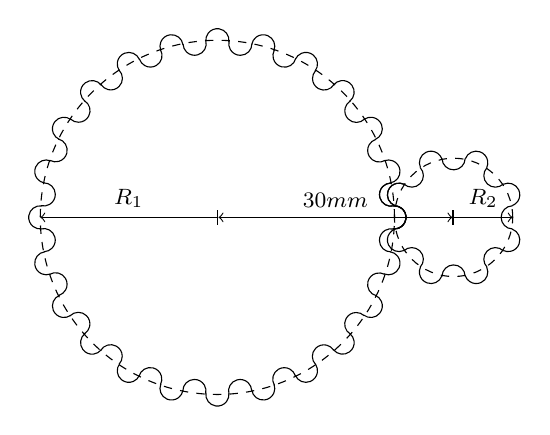
\begin{tikzpicture}[x=1mm,y=1mm]
		\coordinate (m1) at (0,0);
		\coordinate (m2) at (30,0);
		%\path (m1)  + ({22.49085405 * cos(0)},{22.49085405 * sin(0)}) arc[radius = 22.49085405, start angle=0,end angle =360] coordinate[pos=0] (km1) ;
		\draw[dashed] (m1)  + ({22.49085405 * cos(0)},{22.49085405 * sin(0)}) arc[radius = 22.49085405, start angle=0,end angle =360] coordinate[pos={8/360}] (km2) ;
		\draw[dashed] (m2)  + ({7.508037642 * cos(0)},{7.508037642 * sin(0)}) arc[radius = 7.508037642, start angle=0,end angle =360] ;
		%big gear
		\foreach \i in {0,1, ...,24}{
			\begin{scope}[rotate around={\i*15:(m1)}]
			%nach aussen
			\draw (22.49196236,0) + ({1.471832758 * cos(-97.87500000)},{1.471832758 * sin(-97.87500000)}) arc[radius=1.471832758,start angle = -97.87500000,end angle = 95.87500000];
			%nach innen
			\draw ({22.49196236*cos(7.5)},{22.49196236*sin(7.5)}) + ({1.471832758 * cos(-84)},{1.471832758 * sin(-84)}) arc[radius=1.471832758,start angle = -74.37500000,end angle = -268.125];
			\end{scope}
		}
		
		%small gear
		\foreach \i in {0,1, ...,8}{
			\begin{scope}[rotate around={\i*45:(m2)}]
			%nach aussen
			\draw (22.49196236,0) + ({1.471832758 * cos(-88.62500000)},{1.471832758 * sin(-88.62500000)}) arc[radius=1.471832758,start angle = -88.62500000,end angle = 88.62500000];
			%nach innen
			\draw (m2) ++ ({180-45/2}:7.508037642) ++ ({1.471832758 * cos(-110.12500000)},{1.471832758 * sin(-110.12500000)}) arc[radius=1.471832758,start angle = -110.12500000,end angle = -294.875];
			\end{scope}
		}
		
		
		%radii
		\draw[->] (m1) -- +(-22.49196236,0) node[pos=0.5,above] {\footnotesize$R_1$};
		\draw[->] (m2) -- +(7.508037642,0) node[pos=0.5,above] {\footnotesize$R_2$};
		
		\draw[|<->|] (m1) -- +(m2) node[pos=0.5,above] {\footnotesize$30mm$};
		
		
		\end{tikzpicture}
		\caption{Resulting Gears}
	\end{figure}
	
	
	\myexample{Internal ring gear}
	A internal ring gear $K_r$ with outer diameter $D_r = 5$ should be calculated such that a smaller gear $K$ can be used to archive a $5:1$  gear reduction. The two shafts should be $15mm$ apart.\\
	As the two shafts are $15mm$ apart we know that
	\begin{align*}
		R_r-R=15.
	\end{align*}
	Furthermore 
	\begin{align*}
		n_r = 5\cdot n
	\end{align*} 
	to achieve the required $5:1$ ratio.
		Using \cref{eq:R-r} we also know that:
	\begin{align*}
	\varphi_r &= \frac{2\pi}{n_r}\\
	R_r&= \frac{r*\cos\left( \frac{\varphi_r }{4}\right) }{\sin(\frac{\varphi_r}{2})}\\
	\varphi&= \frac{2\pi}{n}\\
	R&= \frac{r*\cos\left( \frac{\varphi }{4}\right) }{\sin(\frac{\varphi}{2})}
	\end{align*}
	If we specify the number of teeth on either one of them lets say
	\begin{align*}
	n=8,
	\end{align*}
	we can solve the system of equations using wolframalpha, maple or another computerprogram to find a unique solution. In this example we get:
	\begin{align*}
	r &= 1.474527091\\
	R_r &= 18.77908826\\
	R &= 3.779088256\\
	n_r &= 40\\
	n &= 8\\
	\varphi_r &= 0.1570796327\\
	\varphi &= 0.7853981635
	\end{align*}
	

	\begin{figure}[H]
		\begin{subfigure}[t]{0.5\textwidth}
			\centering
			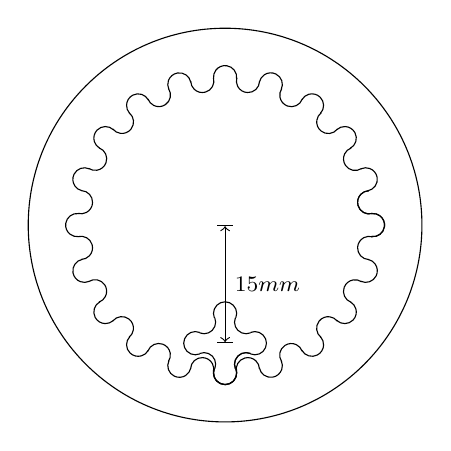
\begin{tikzpicture}[x=1mm,y=1mm]
			\coordinate (m1) at (0,0);
			\coordinate (m2) at (0,-15);
			%\path (m1)  + ({22.49085405 * cos(0)},{22.49085405 * sin(0)}) arc[radius = 22.49085405, start angle=0,end angle =360] coordinate[pos=0] (km1) ;
			%\draw[dashed] (m1)  + ({22.49085405 * cos(0)},{22.49085405 * sin(0)}) arc[radius = 22.49085405, start angle=0,end angle =360] coordinate[pos={8/360}] (km2) ;
			%\draw[dashed] (m2)  + ({7.508037642 * cos(0)},{7.508037642 * sin(0)}) arc[radius = 7.508037642, start angle=0,end angle =360] ;
			
			\draw (m1)  + ({25 * cos(0)},{25 * sin(0)}) arc[radius = 25, start angle=0,end angle =360] ;
			%big gear
			\foreach \i in {0,1, ...,20}{
				\begin{scope}[rotate around={\i*18:(m1)}]
				%nach aussen
				\draw (18.77908826,0) + ({1.4745270918 * cos(-97.87500000)},{1.474527091* sin(-97.87500000)}) arc[radius=1.474527091,start angle = -97.87500000,end angle = 95.87500000];
				%nach innen
				\draw ({18.77908826*cos(9)},{18.77908826*sin(9)}) + ({1.474527091 * cos(-84)},{1.474527091 * sin(-84)}) arc[radius=1.474527091,start angle = -74.37500000,end angle = -268.125];
				\end{scope}
			}
			
			%small gear
			\foreach \i in {0,1, ...,4}{
				\begin{scope}[rotate around={\i*90:(m2)}]
				%nach aussen
				\draw (m2) ++ (-90:3.779088256) ++ ({1.474527091 * cos(-202.5)},{1.474527091 * sin(-202.5)}) arc[radius=1.474527091,start angle = -202.5,end angle = 22.5];
				%nach innen
				\draw (m2) ++ ({-90+45}:3.779088256) ++ ({1.474527091 * cos(67.5)},{1.474527091 * sin(67.5)}) arc[radius=1.474527091,start angle = 67.5,end angle = 202.5];
				\end{scope}
			}
			%radii
			\draw[|<->|] (m1) -- +(m2) node[pos=0.5,right] {\footnotesize$15mm$};
			
			
			\end{tikzpicture}
			\subcaption{$n=8$}
			\label{fig:precond-vs-cg}	
		\end{subfigure}
		\begin{subfigure}[t]{0.5\textwidth}
			\centering
			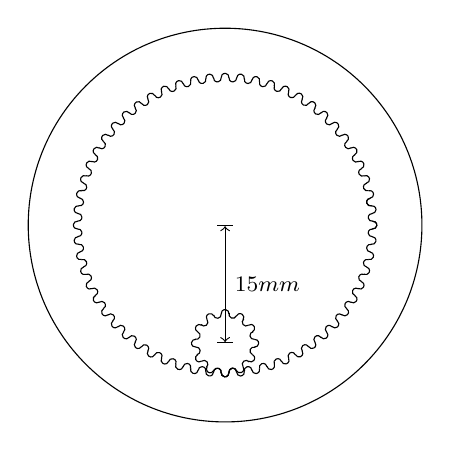
\begin{tikzpicture}[x=1mm,y=1mm]
			\coordinate (m1) at (0,0);
			\coordinate (m2) at (0,-15);
			%\path (m1)  + ({22.49085405 * cos(0)},{22.49085405 * sin(0)}) arc[radius = 22.49085405, start angle=0,end angle =360] coordinate[pos=0] (km1) ;
			%\draw[dashed] (m1)  + ({22.49085405 * cos(0)},{22.49085405 * sin(0)}) arc[radius = 22.49085405, start angle=0,end angle =360] coordinate[pos={8/360}] (km2) ;
			%\draw[dashed] (m2)  + ({7.508037642 * cos(0)},{7.508037642 * sin(0)}) arc[radius = 7.508037642, start angle=0,end angle =360] ;
			
			\draw (m1)  + ({25 * cos(0)},{25 * sin(0)}) arc[radius = 25, start angle=0,end angle =360] ;
			%big gear
			\foreach \i in {0,1, ...,60}{
				\begin{scope}[rotate around={\i*6:(m1)}]
				%nach aussen
				\draw (18.77908826,0) + ({.4909439976 * cos(-97.87500000)},{.4909439976* sin(-97.87500000)}) arc[radius=.4909439976,start angle = -97.87500000,end angle = 95.87500000];
				%nach innen
				\draw ({18.77908826*cos(9)},{18.77908826*sin(9)}) + ({.4909439976 * cos(-84)},{.4909439976 * sin(-84)}) arc[radius=.4909439976,start angle = -74.37500000,end angle = -268.125];
				\end{scope}
			}
			
			%small gear
			\foreach \i in {0,1, ...,12}{
				\begin{scope}[rotate around={\i*30:(m2)}]
				%nach aussen
				\draw (m2) ++ (-90:3.779088256) ++ ({.4909439976 * cos(-187.5)},{.4909439976 * sin(-187.5)}) arc[radius=.4909439976,start angle = -187.5,end angle = 7.5];
				%nach innen
				\draw (m2) ++ ({-90+15}:3.779088256) ++ ({.4909439976 * cos(7.5)},{.4909439976 * sin(7.5)}) arc[radius=.4909439976,start angle = 7.5,end angle = 187.5];
				\end{scope}
			}
			%radii
			\draw[|<->|] (m1) -- +(m2) node[pos=0.5,right] {\footnotesize$15mm$};
			
			
			\end{tikzpicture}
			\subcaption{$n=24$}
			\label{fig:precond-vs-cg-ndiag}	
		\end{subfigure}
		
		\caption{Resulting internal ring gears for different $n$}\label{fig:internal-ring-gear}
	\end{figure}
	
	
	\myexample{Planetary gearbox (epicyclic gear train)}
	A planetary gearbox with not rotating ring gear and a gear ratio of 5:1 should be calculated.
	Let $S$ be the sun gear, $P$ the planet gear and $R$ the outer ring gear and $C$ the carrier.\\
	We know that for planetary gear systems
	\begin{align*}
		n_R=2\cdot n_P+n_S \implies \frac{n_S}{n_P}\omega _{S}+(2+\frac{n_S}{n_P})\omega _{R}-2(1+\frac{n_S}{n_P})\omega _{C}=0
	\end{align*} 
	where $\omega$ denotes the angular momentum. As the the outer ring gear $R$ is not rotating $\omega_R=0$. We can deduce that 
	\begin{align*}
		\frac{n_S}{n_P}\omega _{S} &= 2(1+\frac{n_S}{n_P})\omega _{C}\\
		\frac{\omega_S}{\omega_C}&=\frac{2(1+\frac{n_S}{n_P})}{\frac{n_S}{n_P}}.
	\end{align*}
	As $S$ will be used as the input and $C$ as the output we know that
	\begin{align*}
		\frac{\omega_S}{\omega_C} = \frac{5}{1}
	\end{align*}
	and because the gears need to touch each other the radii have to satisfy
	\begin{align*}
		R_R=2\cdot R_P+R_S.
	\end{align*}
	We will use \cref{eq:R-r} to get one more equation per gear.\footnote{Take a look at \cref{ex:circ} to see this step in more detail.} After specifying the radius of the outer ring gear $R_R=30$ and $n_S=24$ we can solve the system of equation to get a unique solution. Since we want $4$ planet gears, the sun gear and the outer ring gear have to be symmetrical in both the $x$ and $y$ direction. This is guaranteed if $4\mid n_S$.
		
	\begin{figure}[H]
		\centering
		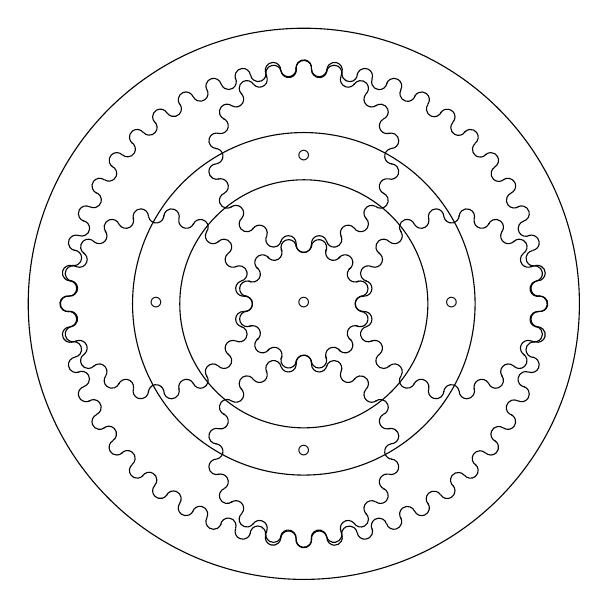
\begin{tikzpicture}[x=1mm,y=1mm]
			\coordinate (m1) at (0,0);
			\coordinate (m2) at (0,-15);
			%\path (m1)  + ({22.49085405 * cos(0)},{22.49085405 * sin(0)}) arc[radius = 22.49085405, start angle=0,end angle =360] coordinate[pos=0] (km1) ;
			%\draw[dashed] (m1)  + ({22.49085405 * cos(0)},{22.49085405 * sin(0)}) arc[radius = 22.49085405, start angle=0,end angle =360] coordinate[pos={8/360}] (km2) ;
			%\draw[dashed] (m2)  + ({7.508037642 * cos(0)},{7.508037642 * sin(0)}) arc[radius = 7.508037642, start angle=0,end angle =360] ;
			
			\draw (m1)++(35,0) arc[radius = 35, start angle=0,end angle =360] ;
			%ring gear
			\foreach \i in {0,1, ...,47}{
				\begin{scope}[rotate around={\i*7.5:(m1)}]
				%nach aussen
				\draw (29.93575886,0) + ({.9813388677 * cos(-97.87500000)},{.9813388677* sin(-97.87500000)}) arc[radius=.9813388677,start angle = -97.87500000,end angle = 95.87500000];
				%nach innen
				\draw ({29.93575886*cos(3.75)},{29.93575886*sin(3.75)}) + ({.9813388677 * cos(-84)},{.9813388677 * sin(-84)}) arc[radius=.9813388677,start angle = -74.37500000,end angle = -268.125];
				\end{scope}
			}
		
			%sun gear
			\begin{scope}[rotate around={15:(0,0)}]
				\foreach \i in {0,1, ...,11}{
					\begin{scope}[rotate around={\i*30:(m1)}]
					%nach aussen
					\draw (7.503214167,0) + ({.9813388677 * cos(-110)},{.9813388677* sin(-105)}) arc[radius=.9813388677,start angle = -105,end angle = 105];
					%nach innen
					\draw ({7.503214167*cos(15)},{7.503214167*sin(15)}) + ({.9813388677 * cos(-75)},{.9813388677 * sin(-75)}) arc[radius=.9813388677,start angle = -75,end angle = -255];
					\end{scope}
				}
			\end{scope}
		
		
			\foreach \i in {0,1, ...,3}{
				
				\node at (0+\i*90:18.751607087) {$\circ$};
				
				\begin{scope}[rotate around={\i*90:(m1) }]
				%planet gear
				\foreach \i in {0,1, ...,17}{
					\begin{scope}[rotate around={\i*20:(-90:18.751607087) }]
					%nach aussen	
					\draw (-90:18.751607087) ++ (-90:11.24839292) ++ ({.9813388677 * cos(-190)},{.9813388677 * sin(-190)}) arc[radius=.9813388677,start angle = -190,end angle = 10];
					%nach innen
					\draw (-90:18.751607087) ++ ({-90+10}:11.24839292) ++ ({.9813388677 * cos(20)},{.9813388677 * sin(20)}) arc[radius=.9813388677,start angle = 20,end angle = 190];
					\end{scope}
				}
				\end{scope}
			}
		
		
		%carrier
		\draw (m1)++(21.751607087,0) arc[radius = 21.751607087, start angle=0,end angle =360] ;
		\draw (m1)++(15.751607087,0) arc[radius = 15.751607087, start angle=0,end angle =360] ;
		
		%center point
		\node at (0,0) {$\circ$};
		
		
		\end{tikzpicture}
		\caption{Resulting planetary gear system}
	\end{figure}

	
	
	\myexample{Rectangular/square gear with given side length}
	A square gear with side length $s=22mm$ should be calculated.\\
	We choose $r=22/12$ according to \cref{therem-rectangle} such that $4r\mid s$.
	Now, as 
	\begin{align*}
		r = \frac{2s}{2n}
	\end{align*}
	we can calculate the number of teeth required as
	\begin{align*}
		n = \frac{s}{r}.
	\end{align*}
	Thus $n = 12$. Note that each corner of the square/rectangle is a center-point of one of the $2n$ circles required to construct the gear.\\
	Depending on whether we want the corners to be teeth or slots in between two teeth, two different gear outlines are possible. The possible gears for this example can be seen in \cref{fig:rectangular-gear}. \Cref{fig:rectangular-gear-smaller-r} shows the resulting gears when using a smaller teeth-size $r=22/24$.
	
	\begin{figure}[h!]
		\begin{subfigure}[t]{0.5\textwidth}
		\centering
		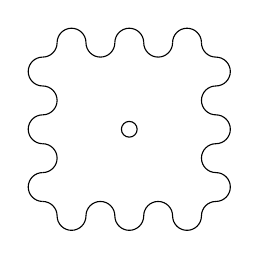
\begin{tikzpicture}[x=1mm,y=1mm]
			\coordinate (m1) at (0,0);
			
			\draw (m1)  + ({1 * cos(0)},{1 * sin(0)}) arc[radius = 1, start angle=0,end angle =360] ;
			
			\foreach \i in {0,1, ...,3}{
				\begin{scope}[rotate around={\i*90:(m1)}]
						\draw ({-11 + 4*1.833333*0},-11) + ({1.833333 * cos(0)},{1.833333 * sin(0)}) arc[radius=1.833333,start angle = 0,end angle = 90];
						\draw ({-11 + 2*1.833333 + 4*1.833333*0},-11) + ({1.833333 * cos(0)},{1.833333 * sin(0)}) arc[radius=1.833333,start angle = 0,end angle = -180];
						\foreach \j in {1,2, ...,2}{
							\draw ({-11 + 4*1.833333*\j},-11) + ({1.833333 * cos(0)},{1.833333 * sin(0)}) arc[radius=1.833333,start angle = 0,end angle = 180];
							\draw ({-11 + 2*1.833333 + 4*1.833333*\j},-11) + ({1.833333 * cos(0)},{1.833333 * sin(0)}) arc[radius=1.833333,start angle = 0,end angle = -180];
						}
				\end{scope}
			}
		\end{tikzpicture}
		\subcaption{Corners are not teeth}
		\end{subfigure}
	\begin{subfigure}[t]{0.5\textwidth}
	\centering
	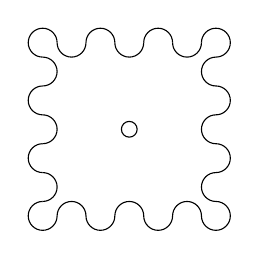
\begin{tikzpicture}[x=1mm,y=1mm]
		\coordinate (m1) at (0,0);
		
		\draw (m1)  + ({1 * cos(0)},{1 * sin(0)}) arc[radius = 1, start angle=0,end angle =360] ;
		
		\foreach \i in {0,1, ...,3}{
			\begin{scope}[rotate around={\i*90:(m1)}]
				\draw ({-11 + 4*1.833333*0},11) + ({1.833333 * cos(0)},{1.833333 * sin(0)}) arc[radius=1.833333,start angle = 0,end angle = 270];
				\draw ({-11 + 2*1.833333 + 4*1.833333*0},11) + ({1.833333 * cos(0)},{1.833333 * sin(0)}) arc[radius=1.833333,start angle = 0,end angle = -180];
				\foreach \j in {1,2, ...,2}{
				\draw ({-11 + 4*1.833333*\j},11) + ({1.833333 * cos(0)},{1.833333 * sin(0)}) arc[radius=1.833333,start angle = 0,end angle = 180];
				\draw ({-11 + 2*1.833333 + 4*1.833333*\j},11) + ({1.833333 * cos(0)},{1.833333 * sin(0)}) arc[radius=1.833333,start angle = 0,end angle = -180];
				}
			\end{scope}
		}
	\end{tikzpicture}
	\subcaption{Corners are teeth}
	\end{subfigure}
	\caption{Resulting rectangular gear for $r=22/12$}\label{fig:rectangular-gear}
	\end{figure}
	
	\begin{figure}[h!]
		\begin{subfigure}[t]{0.5\textwidth}
			\centering
			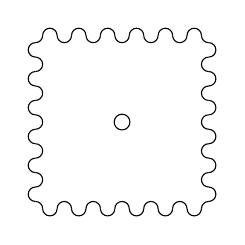
\begin{tikzpicture}[x=1mm,y=1mm]
				\coordinate (m1) at (0,0);
				
				\draw (m1)  + ({1 * cos(0)},{1 * sin(0)}) arc[radius = 1, start angle=0,end angle =360] ;
				
				\foreach \i in {0,1, ...,3}{
					\begin{scope}[rotate around={\i*90:(m1)}]
						\draw ({-11 + 4*1.833333/2*0},-11) + ({1.833333/2 * cos(0)},{1.833333/2 * sin(0)}) arc[radius=1.833333/2,start angle = 0,end angle = 90];
						\draw ({-11 + 2*1.833333/2 + 4*1.833333/2*0},-11) + ({1.833333/2 * cos(0)},{1.833333/2 * sin(0)}) arc[radius=1.833333/2,start angle = 0,end angle = -180];
						\foreach \j in {1,2, ...,5}{
							\draw ({-11 + 4*1.833333/2*\j},-11) + ({1.833333/2 * cos(0)},{1.833333/2 * sin(0)}) arc[radius=1.833333/2,start angle = 0,end angle = 180];
							\draw ({-11 + 2*1.833333/2 + 4*1.833333/2*\j},-11) + ({1.833333/2 * cos(0)},{1.833333/2 * sin(0)}) arc[radius=1.833333/2,start angle = 0,end angle = -180];
						}
					\end{scope}
				}
			\end{tikzpicture}
			\subcaption{Corners are not teeth}
		\end{subfigure}
		\begin{subfigure}[t]{0.5\textwidth}
			\centering
			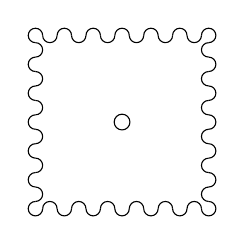
\begin{tikzpicture}[x=1mm,y=1mm]
				\coordinate (m1) at (0,0);
				
				\draw (m1)  + ({1 * cos(0)},{1 * sin(0)}) arc[radius = 1, start angle=0,end angle =360] ;
				
				\foreach \i in {0,1, ...,3}{
					\begin{scope}[rotate around={\i*90:(m1)}]
						\draw ({-11 + 4*1.833333/2*0},11) + ({1.833333/2 * cos(0)},{1.833333/2 * sin(0)}) arc[radius=1.833333/2,start angle = 0,end angle = 270];
						\draw ({-11 + 2*1.833333/2 + 4*1.833333/2*0},11) + ({1.833333/2 * cos(0)},{1.833333/2 * sin(0)}) arc[radius=1.833333/2,start angle = 0,end angle = -180];
						\foreach \j in {1,2, ...,5}{
							\draw ({-11 + 4*1.833333/2*\j},11) + ({1.833333/2 * cos(0)},{1.833333/2 * sin(0)}) arc[radius=1.833333/2,start angle = 0,end angle = 180];
							\draw ({-11 + 2*1.833333/2 + 4*1.833333/2*\j},11) + ({1.833333/2 * cos(0)},{1.833333/2 * sin(0)}) arc[radius=1.833333/2,start angle = 0,end angle = -180];
						}
					\end{scope}
				}
			\end{tikzpicture}
			\subcaption{Corners are teeth}
		\end{subfigure}
		\caption{Resulting rectangular gear for $r=22/24$}\label{fig:rectangular-gear-smaller-r}
	\end{figure}

	\myexample{Rectangular and circular gears with given gear ratio and center-distance}
	A square gear $S$ and a circular gear $C$ that fit together should be calculated given a center-distance $d = 15mm$. \\
	We start building a system of equation:\\
	For $S$ and $C$ to fit together we know that $r_S=r_C$. W therefore use $r=r_S=r_C$ below.
	Given the center-distance $d=15mm$ leads to
	\begin{align*}
		\frac{s}{2} + R_C = 15mm.
	\end{align*}
	Using \cref{theorem-circle} with $\varphi = \pi/(2n_C)$, we get
	\begin{align*}
		R_C = \frac{r\cdot \cos\left(\frac{\varphi}{2}\right)}{\sin \left(\varphi\right)}.
	\end{align*}
	Furthermore, using \cref{therem-rectangle} we know that
	\begin{align*}
		r=\frac{s}{n_S}.
	\end{align*}
	As both $n_S$ and $n_C$ have to be integers we use the symmetry of $C$ to deduce that
	\begin{align*}
		n_S = 2kn_C\quad k\in\mathbb{N}.
	\end{align*}
	We can choose $k$ in a way that the resulting gear and tooth size satisfies our needs. For this example let $k=1$. Therefore $n_S = 2n_C$.\\
	For $C$ to be symmetric we use
	\begin{align*}
		n_C = 12
	\end{align*}
	as our final equation. Solving this system of equations (numerically) results in:
	
	\begin{align*}
		r &= 0.7635571812\\
		R &= 5.837313828\\
		s &= 18.32537235\\
		n_C &= 12\\
		n_S &= 24.
	\end{align*}
	
	The resulting gears can be seen in \cref{fig:square-and-circ-gear} below.

	\begin{figure}[h!]
			\centering
			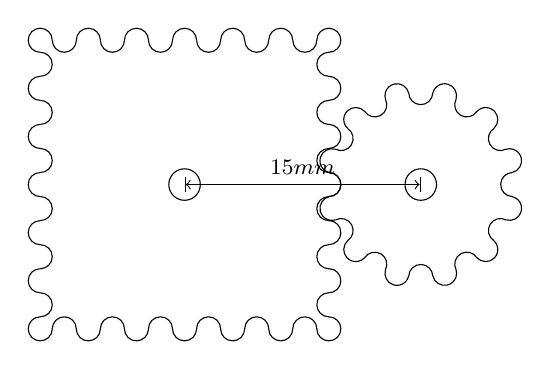
\begin{tikzpicture}[x=1mm,y=1mm,scale=2]
				\coordinate (m1) at (0,0);
				\coordinate (m2) at (15,0);
				
				\draw (m1)  + ({1 * cos(0)},{1 * sin(0)}) arc[radius = 1, start angle=0,end angle =360] ;
				\draw (m2)  + ({1 * cos(0)},{1 * sin(0)}) arc[radius = 1, start angle=0,end angle =360] ;
				
				\foreach \i in {0,1, ...,3}{
					\begin{scope}[rotate around={\i*90:(m1)}]
						\draw ({-9.162686175 + 4*.7635571812*0},9.162686175) + ({.7635571812 * cos(0)},{.7635571812 * sin(0)}) arc[radius=.7635571812,start angle = 0,end angle = 270];
						\draw ({-9.162686175 + 2*.7635571812 + 4*.7635571812*0},9.162686175) + ({.7635571812 * cos(0)},{.7635571812 * sin(0)}) arc[radius=.7635571812,start angle = 0,end angle = -180];
						\foreach \j in {1,2, ...,5}{
							\draw ({-9.162686175 + 4*.7635571812*\j},9.162686175) + ({.7635571812 * cos(0)},{.7635571812 * sin(0)}) arc[radius=.7635571812,start angle = 0,end angle = 180];
							\draw ({-9.162686175 + 2*.7635571812 + 4*.7635571812*\j},9.162686175) + ({.7635571812 * cos(0)},{.7635571812 * sin(0)}) arc[radius=.7635571812,start angle = 0,end angle = -180];
						}
					\end{scope}
				}
			
			%small gear
			\foreach \i in {0,1, ...,11}{
				\begin{scope}[rotate around={\i*30:(m2)}]
					%nach aussen
					\begin{scope}[rotate around={15:(m2)}]
					\draw (m2) ++ (90:5.837313828) ++ ({.7635571812 * cos(-2)},{.7635571812 * sin(-2)}) arc[radius=.7635571812,start angle = -2,end angle = 182];
					\end{scope}
					%nach innen
					\draw (m2) ++ (180:5.837313828) ++ ({.7635571812 * cos(88)},{.7635571812 * sin(88)}) arc[radius=.7635571812,start angle = 88,end angle = -88];
				\end{scope}
			}
		
			\draw[|<->|] (m1) -- +(m2) node[pos=0.5,above] {\footnotesize$15mm$};
		
			\end{tikzpicture}
		\caption{Resulting rectangular gear with fitting circular gear (scale 1:2)}\label{fig:square-and-circ-gear}
	\end{figure}

	\myexample{Elliptical gear with given size and number of teeth}\label{ex:ell-gear}
	A gear in the shape of an ellipse $(x/a)^2+(y/b)^2=1$ with $a=30mm$ and $b=15mm$ and $n=12$ teeth should be constructed.\\
	We start with a parametrization 
	\begin{align*}
		\gamma: [0,2\pi)\rightarrow\mathbb{R}^2,\quad t\mapsto\begin{pmatrix}a\cos(t)\\b\sin(t)\end{pmatrix}
	\end{align*}
	of the given ellipse. As $\gamma$ satisfies the requirements of \cref{theorem:non-circular}, \cref{eq:eqsys} can be used to calculate the tooth-size $r$ and the position of each tooth. As the system of equations required consists of $4n=48$ equations we can not list them here in the same way we did in previous examples. The maple code used to solve this system of equations can be found in \cref{appendix:ell-gear-code}.\\
	Solving this system leads to:
	\begin{align*}
		\begin{array}{lll}
				r = 3.024112686,\quad &  & \\
				\varphi_{1} = 0.,\quad & \varphi_{2} = .1990159115,\quad & \varphi_{3} = .1809691691,\\
				\varphi_{4} = .1599940895,\quad & \varphi_{5} = .1430803899,\quad & \varphi_{6} = .1305321589,\\
				\varphi_{7} = .1213147333,\quad & \varphi_{8} = .1145167936,\quad & \varphi_{9} = .1095068588,\\
				\varphi_{10} = .1058685767,\quad & \varphi_{11} = .1033313491,\quad & \varphi_{12} = .1017233388,\\
				\varphi_{13} = .1009429577,\quad & \varphi_{14} = .1009429577,\quad & \varphi_{15} = .1017233388,\\
				\varphi_{16} = .1033313491,\quad & \varphi_{17} = .1058685767,\quad & \varphi_{18} = .1095068588,\\
				\varphi_{19} = .1145167936,\quad & \varphi_{20} = .1213147333,\quad & \varphi_{21} = .1305321589,\\
				\varphi_{22} = .1430803899,\quad & \varphi_{23} = .1599940895,\quad & \varphi_{24} = .1809691691,\\
				\varphi_{25} = .1990159115,\quad & \varphi_{26} = .1990159115,\quad & \varphi_{27} = .1809691691,\\
				\varphi_{28} = .1599940895,\quad & \varphi_{29} = .1430803899,\quad & \varphi_{30} = .1305321589,\\
				\varphi_{31} = .1213147333,\quad & \varphi_{32} = .1145167936,\quad & \varphi_{33} = .1095068588,\\
				\varphi_{34} = .1058685767,\quad & \varphi_{35} = .1033313491,\quad & \varphi_{36} = .1017233388,\\
				\varphi_{37} = .1009429577,\quad & \varphi_{38} = .1009429577,\quad & \varphi_{39} = .1017233388,\\
				\varphi_{40} = .1033313491,\quad & \varphi_{41} = .1058685767,\quad & \varphi_{42} = .1095068588,\\
				\varphi_{43} = .1145167936,\quad & \varphi_{44} = .1213147333,\quad & \varphi_{45} = .1305321589,\\ 
				\varphi_{46} = .1430803899,\quad & \varphi_{47} = .1599940895,\quad & \varphi_{48} = .1809691691
		\end{array}
	\end{align*}
	Note that we do not have to use the parameters $\varphi_i$ when constructing the gear outline. As we now know $r$ we can use a pattern, symmetry, congruence or other techniques to draw the gear in CAD. The result of this example as well as the result using a greater number of teeth can be seen in \cref{fig:ell-gear} below.\\
	Due to the symmetry of $\gamma$ and the fact that $4\mid n$ the resulting gear outline is symmetric along the $x$ and $y$-axis.
	
	\begin{figure}[H]
		\begin{subfigure}[t]{0.5\textwidth}
			\centering
			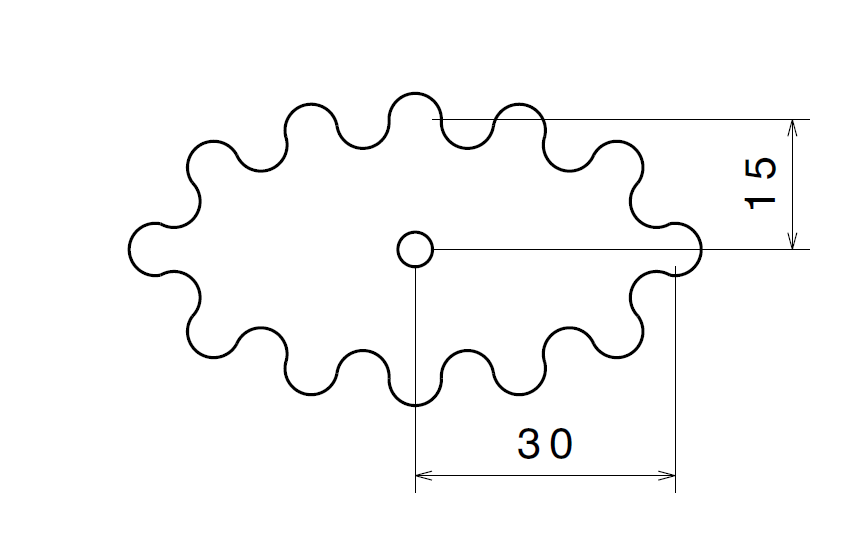
\includegraphics[width=60mm]{ell-gear.png}
			\subcaption{$n=12$}
		\end{subfigure}
		\begin{subfigure}[t]{0.5\textwidth}
			\centering
			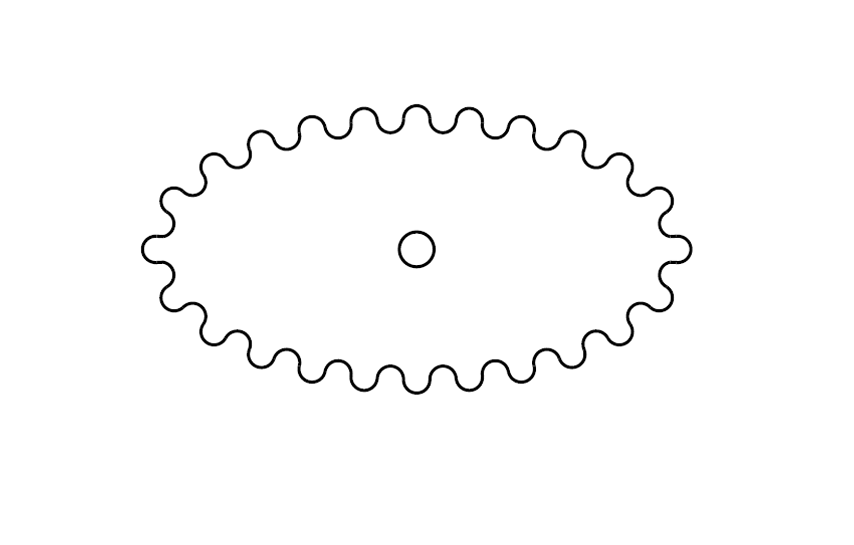
\includegraphics[width=60mm]{ell-gear-fine.png}
			\subcaption{$n=24$}
		\end{subfigure}
		\caption{Resulting elliptical gear with different number of teeth}\label{fig:ell-gear}
	\end{figure}
	\myexample{Elliptical gear and square gear that fit together}
	Given the elliptical gear $E$ constructed in \cref{ex:ell-gear} a fitting square gear $S$ should be calculated.\\
	We recall that $r=1.513379781$ for $n_E=24$. We now choose the side-length $s$ of $S$ according to \cref{therem-rectangle} such that $4r\mid s$.
	Let $s=28r$.\\
	Note that it is very easy to calculate fitting gears if the size of at least one of them is not given.\\
	As we now know $s$ and $r$ we can proceed to calculate $n_S=28$ using (again) the findings of \cref{therem-rectangle}:
	\begin{align*}
		n_S=\frac{s}{r}.
	\end{align*}
	The two resulting gears are shown in \cref{fig:ell-square-gear}.
	
	\begin{figure}[H]
			\centering
			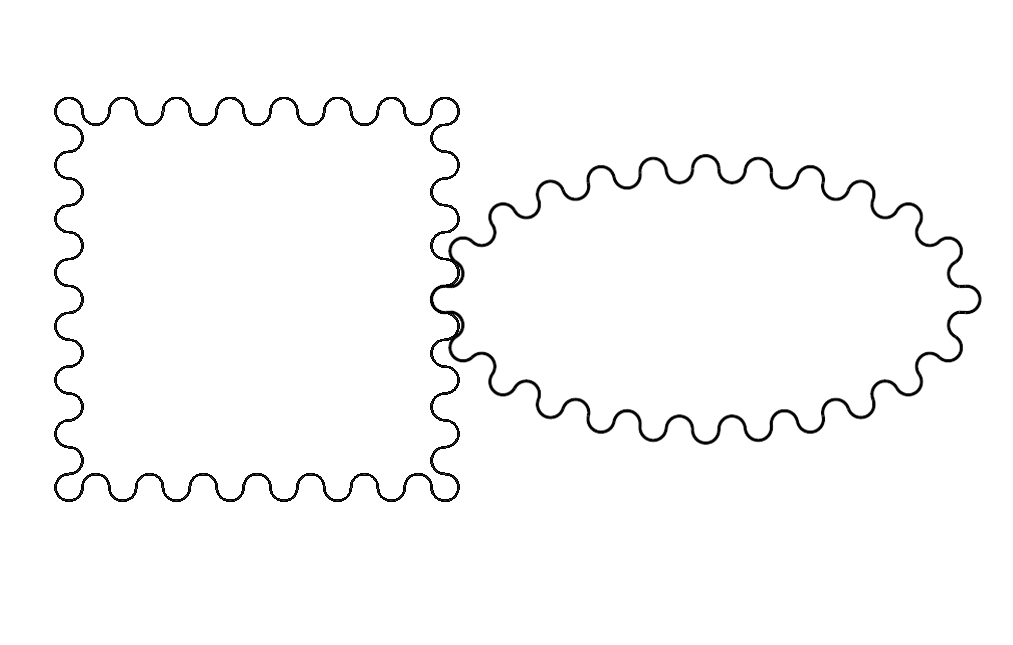
\includegraphics[width=80mm]{ell-square-gear-fine.png}
		\caption{Resulting elliptical gear with fitting square gear}\label{fig:ell-square-gear}
	\end{figure}

	
	\newpage
	\appendix
	\section{Code used in the Examples}\label{appendix:code}
	\subsection{Elliptical gear with given size and number of teeth}\label{appendix:ell-gear-code}
	\lstinputlisting[caption=elliptical gears using maple]{ell-gear.txt}
	\newpage 
	%\printindex
	\thispagestyle{firststyle}
	\newpage
	\printbibliography
	%\newpage
	\listoffigures
	%\thispagestyle{firststyle}
	%\listoftables
	\thispagestyle{firststyle}
	
	\newpage
	\appendix
	\newpage
	
	
\end{document}

